\documentclass{exam}

\usepackage{units} 
\usepackage{graphicx}
\usepackage[fleqn]{amsmath}
\usepackage{cancel}
\usepackage{float}
\usepackage{mdwlist}
\usepackage{booktabs}
\usepackage{cancel}
\usepackage{polynom}
\usepackage{caption}
\usepackage{fullpage}
\usepackage{comment}
\usepackage{enumerate}
\usepackage{xfrac}

\newcommand{\degree}{\ensuremath{^\circ}} 
\everymath{\displaystyle}

\printanswers

% \begin{figure}[H]
%   \centering
%   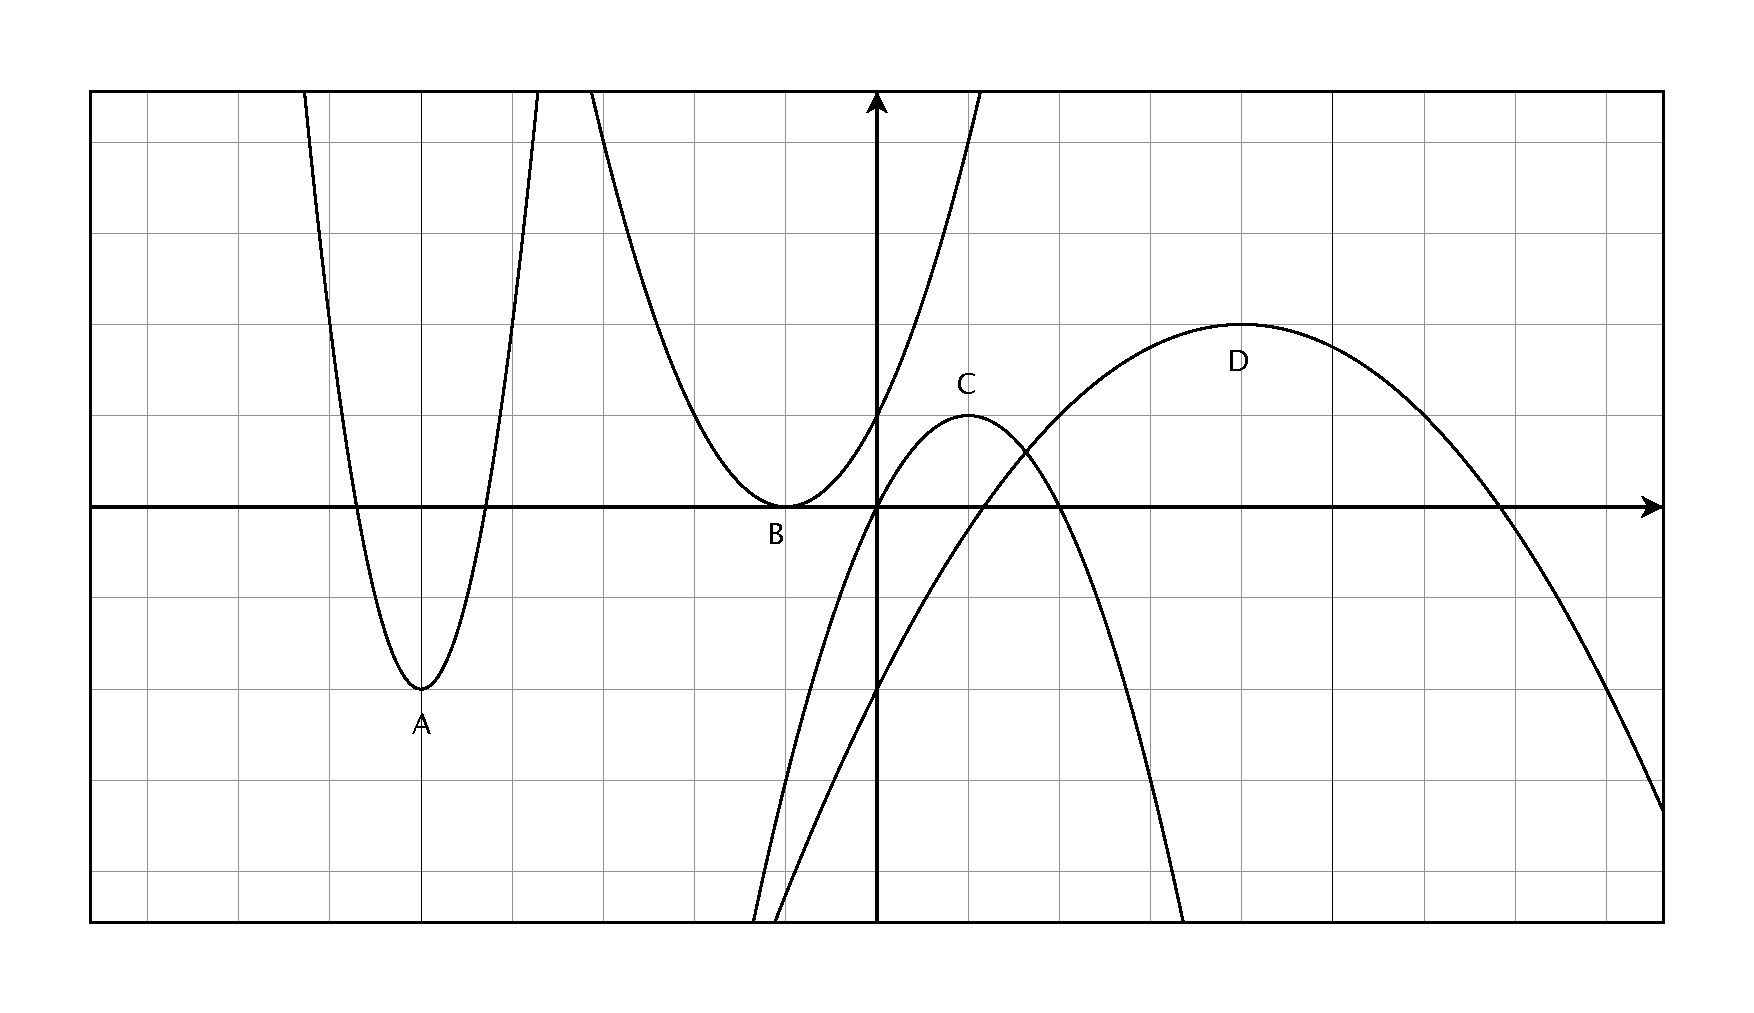
\includegraphics[scale=.3]{problem_7.eps}
%   \caption*{Problem 7}
% \end{figure}

% \begin{tabular}{cc}
% \toprule
% period & amplitude \\
% \midrule
%   $\pi$ & $2$ \\
% \bottomrule
% \end{tabular}

\title{Math 142 Notes \\ Section 5.2}

\date{\today}

\begin{document}

  \maketitle
  \tableofcontents

  \section{Sine/Cosine/Tangent}

  \subsection{Definition}

  On unit circle:
  \begin{itemize*}
    \item sine: y coordinate on unit circle
    \item cosine: x coordinate on unit circle
    \item tangent: $\sfrac{y}{x}$ ($x \neq 0$)
  \end{itemize*}

  \subsection{Examples}

  \begin{itemize*}
    \item fill in table with 0, $\pi$, $\frac{\pi}{2}$, $\frac{\pi}{6}$, $\frac{\pi}{4}$, $\frac{\pi}{3}$ (first
      quadrant only)
    \item examples in all quadrants
    \item show quadrant sign chart for all
    \item unit circle with all values
  \end{itemize*}

  \section{Secant/Cosecant/Cotangent}
  \subsection{Definitions}
  \begin{itemize*}
    \item secant: \sfrac{1}{x} ($x \neq 0$)
    \item cosecant: \sfrac{1}{y} ($y \neq 0$)
    \item cotangent: \sfrac{x}{y} ($y \neq 0$)
  \end{itemize*}

  \subsection{Examples}

  \begin{itemize*}
    \item fill in table with 0, $\pi$, $\frac{\pi}{2}$, $\frac{\pi}{6}$, $\frac{\pi}{4}$, $\frac{\pi}{3}$ (first
      quadrant only)
    \item examples in all quadrants
    \item show quadrant sign chart for all
    \item unit circle with all values
  \end{itemize*}

  \section{Evaluating Trigonometric Functions}

  \subsection{Procedure}
  \begin{itemize*}
    \item find reference number
    \item look up from table or memorize
    \item use appropriate sign for quadrant
  \end{itemize*}

  \subsection{Problems}
  \begin{enumerate}

    \item
      $t = \frac{2 \pi}{3}$

      \begin{tabular}[H]{cccccc}
        \toprule
        $\sin t$             & $\cos t$        & $\tan t$     & $\csc t$             & $\sec t$ & $\cot t$ \\
        \midrule
        $\frac{\sqrt{3}}{2}$ & $- \frac{1}{2}$ & $- \sqrt{3}$ & $\frac{2}{\sqrt{3}}$ & $- 2$    & $- \frac{1}{\sqrt{3}}$ \\
        \bottomrule
      \end{tabular}

    \item
      $t = \frac{7 \pi}{6}$

      \begin{tabular}[H]{cccccc}
        \toprule
        $\sin t$       & $\cos t$               & $\tan t$             & $\csc t$ & $\sec t$               & $\cot t$ \\
        \midrule
        $-\frac{1}{2}$ & $- \frac{\sqrt{3}}{2}$ & $\frac{\sqrt{3}}{3}$ & $-2$     & $- \frac{2}{\sqrt{3}}$ & $\sqrt{3}$ \\
        \bottomrule
      \end{tabular}

    \item
      $t = - \frac{\pi}{4}$

      \begin{tabular}[H]{cccccc}
        \toprule
        $\sin t$               & $\cos t$             & $\tan t$ & $\csc t$    & $\sec t$   & $\cot t$ \\
        \midrule
        $- \frac{\sqrt{2}}{2}$ & $\frac{\sqrt{2}}{2}$ & $-1$     & $-\sqrt{2}$ & $\sqrt{2}$ & $-1$ \\
        \bottomrule
      \end{tabular}

    \item
      $\left( \frac{\sqrt{15}}{4}, - \frac{1}{4} \right)$

      \begin{tabular}[H]{cccccc}
        \toprule
        $\sin t$       & $\cos t$              & $\tan t$               & $\csc t$ & $\sec t$              & $\cot t$ \\
        \midrule
        $-\frac{1}{4}$ & $\frac{\sqrt{15}}{4}$ & $-\frac{1}{\sqrt{15}}$ & $-4$     & $\frac{4}{\sqrt{15}}$ & $-\sqrt{15}$ \\
        \bottomrule
      \end{tabular}

    \item If $\sin t > 0$ and $\tan t < 0$, what quadrant is the terminal point in? (II)

    \item If $\cos t > 0$ and $\sin t < 0$, what quadrant is the terminal point in? (IV)

    \item
      $\cos t > 0$ and $\tan t < 0$, $\tan t = - \frac{3}{4}$


      If $\cos t > 0$ and $\tan t < 0$, the point is in quadrant IV

      \begin{tabular}[H]{cccccc}
        \toprule
        $\sin t$       & $\cos t$      & $\tan t$       & $\csc t$       & $\sec t$      & $\cot t$ \\
        \midrule
        $-\frac{3}{5}$ & $\frac{4}{5}$ & $-\frac{3}{4}$ & $-\frac{5}{3}$ & $\frac{5}{4}$ & $\frac{4}{3}$ \\
        \bottomrule
      \end{tabular}

    \item if $\sin t = \frac{2}{5}$ and $t$ is in quadrant II, find the values of the other trigonometric functions

      \begin{tabular}[H]{cccccc}
        \toprule
        $\sin t$      & $\cos t$        & $\tan t$       & $\csc t$      & $\sec t$       & $\cot t$ \\
        \midrule
        $\frac{2}{5}$ & $- \frac{3}{5}$ & $-\frac{2}{3}$ & $\frac{5}{2}$ & $-\frac{5}{3}$ & $-\frac{3}{2}$ \\
        \bottomrule
      \end{tabular}

    \item
      \[
        \sec t = 2
      \]
      quadrant IV

      \begin{tabular}[H]{cccccc}
        \toprule
        $\sin t$              & $\cos t$      & $\tan t$    & $\csc t$                & $\sec t$ & $\cot t$ \\
        \midrule
        $-\frac{\sqrt{3}}{2}$ & $\frac{1}{2}$ & $-\sqrt{3}$ & $-\frac{2 \sqrt{3}}{3}$ & $2$      & $-\frac{\sqrt{3}}{3}$ \\
        \bottomrule
      \end{tabular}


    \item
      \[
        \tan t = - 4
      \]
      If $\tan t < 0$ and $\csc t > 0$, the point is in quadrant II

      \begin{tabular}[H]{cccccc}
        \toprule
        $\sin t$                 & $\cos t$                & $\tan t$ & $\csc t$              & $\sec t$     & $\cot t$ \\
        \midrule
        $\frac{4 \sqrt{17}}{17}$ & $-\frac{\sqrt{17}}{17}$ & $-4$     & $\frac{\sqrt{17}}{4}$ & $-\sqrt{17}$ & $-\frac{1}{4}$ \\
        \bottomrule
      \end{tabular}

  \end{enumerate}
  Do examples like $\frac{2 \pi}{3}$, $\frac{5 \pi}{4}$, $- \frac{\pi}{2}$, etc.

  % \section{Domains}
  % \begin{tabular}[H]{ll}
  %   $\sin$, $\cos$ & all real numbers \\
  %   $\tan$, $\sec$ & $t \neq \sfrac{\pi}{2} + n \pi$  \\
  %   $\cot$, $\csc$ & $t \neq n \pi$  \\
  % \end{tabular}

  \section{Even/Odd}
  \subsection{Overview}
  \begin{itemize*}
    \item review even/odd definitions
    \item $\sin (-t) = -y = - \sin t$
    \item $\tan (-t) = - \sfrac{y}{x} = - \tan t$
    \item $\cos (-t) = x = \cos t$
    \item sine, cosecant, tangent, and cotangent are odd
    \item cosine and secant are even
  \end{itemize*}

  \subsection{Examples}
  \begin{itemize*}
    \item $\sin (- \sfrac{\pi}{2}) = - \sin \sfrac{\pi}{2} = \sfrac{\sqrt{2}}{2}$
    \item $\cos (- \sfrac{\pi}{2}) = \cos \sfrac{\pi}{2} = \sfrac{\sqrt{2}}{2}$

    \item $\sin x - \cos x$ (neither)
    \item $\sin x \cos x$ (odd)
    \item $x^2 \cos x$ (even)
  \end{itemize*}

  \section{Identities}

  \subsection{Fundamental Identities}
  \begin{itemize*}
    \item secant, etc. inverses of cosine, etc.
    \item $\sin^2 t + \cos^2 t = 1$
    \item $\tan^2 t + 1 = \sec^2 t$
    \item $\cot^2 t + 1 = \csc^2 t$
  \end{itemize*}

  \subsection{Applications}

  \begin{enumerate}
    \item write $\sin t$ in terms of $\cos t$ where $t$ is in quadrant IV
      \begin{align*}
        \sin^2 t + \cos^2 t & = 1 \\
        \sin^2 t            & = 1 - \cos^2 t \\
        \sin t              & = \pm \sqrt{ 1 - \cos^2 t } \\
      \end{align*}

      In quadrant IV, $\sin t = - \sqrt{ 1 - \cos^2 t }$ 

    \item write $\tan t$ in terms of $\cos t$ where $t$ is in quadrant III
      \begin{align*}
        \sec^2 t & = \tan^2 t + 1 \\
        \tan^2 t & = \sec^2 t - 1 \\
        \tan t   & = \pm \sqrt{ \sec^2 t - 1 } \\
        \tan t   & = \pm \sqrt{ \frac{1}{\cos^2 t} - 1 } \\
      \end{align*}

      In quadrant III, $\tan t = \sqrt{ \frac{1}{\cos^2 t} - 1 }$ 

  \end{enumerate}

  \section{Trigonometric Functions as Projections}

  Explain projections as shadows and draw pictures with flashlights and shadow.

  \begin{itemize*}
    \item $\sin$ and $\cos$ are projections of radius on x/y axes
    \item $\tan$ is projection of extension of radius to tangent line at $(1, 0)$ from left (show with similar triangles)
    \item $\sec$ is projection of extension of radius to tangent line at radius intersection point from above on to x
      axis (show with similar triangles)
    \item $\csc$ is projection of extension of radius to tangent line at radius intersection point from right on to y
      axis (show with similar triangles)
  \end{itemize*}
\end{document}
